\documentclass[11pt]{article}
\usepackage[UTF8]{ctex}
\usepackage{subcaption}
%%%%%%%%%%%%%%%%%%%%%%%%%%%%%%%%%%%%%%%%%
% Cleese Assignment
% Structure Specification File
% Version 1.0 (27/5/2018)
%
% This template originates from:
% http://www.LaTeXTemplates.com
%
% Author:
% Vel (vel@LaTeXTemplates.com)
%
% License:
% CC BY-NC-SA 3.0 (http://creativecommons.org/licenses/by-nc-sa/3.0/)
%
%%%%%%%%%%%%%%%%%%%%%%%%%%%%%%%%%%%%%%%%%

%----------------------------------------------------------------------------------------
%	PACKAGES AND OTHER DOCUMENT CONFIGURATIONS
%----------------------------------------------------------------------------------------

\usepackage{lastpage} % Required to determine the last page number for the footer

\usepackage{graphicx} % Required to insert images

\setlength\parindent{0pt} % Removes all indentation from paragraphs

\usepackage[most]{tcolorbox} % Required for boxes that split across pages

\usepackage{booktabs} % Required for better horizontal rules in tables

\usepackage{listings} % Required for insertion of code

\usepackage{etoolbox} % Required for if statements

\usepackage{amsmath}
\usepackage{amsthm}
\usepackage{amssymb}
\usepackage{indentfirst}
\usepackage{diagbox}
\usepackage{subfigure}
\usepackage{float}
\usepackage{xcolor}
\usepackage[colorlinks, linkcolor = black]{hyperref}

\usepackage{enumerate}
\usepackage{enumitem}
\setlist{
    leftmargin = .1\linewidth,
    % rightmargin = .1\linewidth,
    % label=\emph{\alph*}.
}

\setlength{\parindent}{2em}

\usepackage{siunitx}
\sisetup
{
    output-exponent-marker = \ensuremath{\mathrm{E}},
    exponent-product = {},
    retain-explicit-plus,
    retain-zero-exponent,
}
%----------------------------------------------------------------------------------------
%	MARGINS
%----------------------------------------------------------------------------------------

\usepackage{geometry} % Required for adjusting page dimensions and margins

\geometry{
    paper=a4paper, % Change to letterpaper for US letter
    top=3cm, % Top margin
    bottom=3cm, % Bottom margin
    left=2.5cm, % Left margin
    right=2.5cm, % Right margin
    headheight=14pt, % Header height
    footskip=1.4cm, % Space from the bottom margin to the baseline of the footer
    headsep=1.2cm, % Space from the top margin to the baseline of the header
    %showframe, % Uncomment to show how the type block is set on the page
}

%----------------------------------------------------------------------------------------
%	FONT
%----------------------------------------------------------------------------------------

\usepackage[utf8]{inputenc} % Required for inputting international characters
\usepackage[T1]{fontenc} % Output font encoding for international characters

% \usepackage[sfdefault,light]{roboto} % Use the Roboto font

%----------------------------------------------------------------------------------------
%	HEADERS AND FOOTERS
%----------------------------------------------------------------------------------------

\usepackage{fancyhdr} % Required for customising headers and footers

\pagestyle{fancy} % Enable custom headers and footers

\lhead{\small\assignmentClass} % Left header; output the instructor in brackets if one was set
\chead{\small\assignmentTitle} % Centre header
\rhead{\small\ifdef{\assignmentAuthorName}{\assignmentAuthorName}{\ifdef{\assignmentDate}{Due\ \assignmentDate}{}}} % Right header; output the author name if one was set, otherwise the due date if that was set

\lfoot{} % Left footer
\cfoot{\small Page\ \thepage\ of\ \pageref{LastPage}} % Centre footer
\rfoot{} % Right footer

\renewcommand\headrulewidth{0.5pt} % Thickness of the header rule

%----------------------------------------------------------------------------------------
%	MODIFY SECTION STYLES
%----------------------------------------------------------------------------------------

\usepackage{titlesec} % Required for modifying sections

%------------------------------------------------
% Section

\titleformat
{\section} % Section type being modified
[block] % Shape type, can be: hang, block, display, runin, leftmargin, rightmargin, drop, wrap, frame
{\Large\bfseries} % Format of the whole section
{\arabic{section}} % Format of the section label
{6pt} % Space between the title and label
{} % Code before the label

\titlespacing{\section}{0pt}{0.5\baselineskip}{0.5\baselineskip} % Spacing around section titles, the order is: left, before and after

%------------------------------------------------
% Subsection

\titleformat
{\subsection} % Section type being modified
[block] % Shape type, can be: hang, block, display, runin, leftmargin, rightmargin, drop, wrap, frame
{\itshape} % Format of the whole section
{(\arabic{subsection})} % Format of the section label
{4pt} % Space between the title and label
{} % Code before the label

\titlespacing{\subsection}{0pt}{0.5\baselineskip}{0.5\baselineskip} % Spacing around section titles, the order is: left, before and after

\renewcommand\thesubsection{(\arabic{subsection})}

%----------------------------------------------------------------------------------------
%	CUSTOM QUESTION COMMANDS/ENVIRONMENTS
%----------------------------------------------------------------------------------------



% Command to print an assignment section title to split an assignment into major parts
\newcommand{\assignmentSection}[1]{
    \newpage
    {
        \centering % Centre the section title
        \vspace{2\baselineskip} % Whitespace before the entire section title

        \rule{0.8\textwidth}{0.5pt} % Horizontal rule

        \vspace{0.75\baselineskip} % Whitespace before the section title
        {\LARGE \textsc{#1}} % Section title, forced to be uppercase

        \rule{0.8\textwidth}{0.5pt} % Horizontal rule

        \vspace{\baselineskip} % Whitespace after the entire section title
    }
    \setcounter{section}{0}

}

%----------------------------------------------------------------------------------------
%	TITLE PAGE
%----------------------------------------------------------------------------------------

\author{\textbf{\assignmentNo\ \assignmentAuthorName}} % Set the default title page author field
\date{} % Don't use the default title page date field

\title{
    \thispagestyle{empty} % Suppress headers and footers
    \vspace{0.2\textheight} % Whitespace before the title
    \textbf{\assignmentClass}\\[5pt]
    \texttt{\assignmentTitle}\\[-4pt]
    % \ifdef{\assignmentSubTitle}{\texttt{\assignmentSubTitle}}{}
    \ifdef{\assignmentDate}{\assignmentDate}{} % If a due date is supplied, output it
    \ifdef{\assignmentClassInstructor}{{\large \textit{\assignmentClassInstructor}}}{} % If an instructor is supplied, output it
    \vspace{0.32\textheight} % Whitespace before the author name
}
 % Include the file specifying the document structure and custom commands

\sisetup
{
    table-format = +1.12e+003,
}

\newcommand{\assignmentQuestionName}{Question} % The word to be used as a prefix to question numbers; example alternatives: Problem, Exercise
\newcommand{\assignmentClass}{计算方法B} % Course/class
\newcommand{\assignmentTitle}{Programming Assignment\ \#3}
\newcommand{\assignmentDate}{2020.4.20} % date
\newcommand{\assignmentNo}{PB17000297}
\newcommand{\assignmentAuthorName}{罗晏宸} % Student name

\begin{document}

\maketitle % Print the title page

\thispagestyle{empty} % Suppress headers and footers on the title page

\newpage

\assignmentSection{非线性方程求根}
\section{问题描述}
分别编写用 Newton 法和弦截法求根的通用程序。再利用你的通用程序分别求下面方程的根
$$
    f(x) = 2x^4 + 24x^3 + 61x - 16x + 1 = 0
$$
其中, Newton 迭代法分别取初值 $x_0 = 0$ 和 $x_0 = 3$;弦截法的初值分别取为 $x_0 = 0,\ x_1 = 0.5$ 以及 $x_0 = 0.1,\ x_1 = 1.5$;

取误差限$\varepsilon$为\num{1.0e-9},即当$|f(x_k)| < \varepsilon$时,停止迭代。将计算结果列成表格,要求给出初值、每步的迭代结果,以及最终的迭代结果(包括迭代步数);比较或分析两种计算方法的优劣。

\section{计算结果}
\begin{figure}
    \centering
    \begin{subfigure}[t]{\textwidth}
        \centering
        \begin{tabular}{|l|c|c|}
            \hline
            迭代步数$k$            & $x_k$                        & $f(x_k)$                     \\
            \hline $k = 0$(初值) & $0.0000000000\text{E}{+}000$ & $1.0000000000\text{E}{+}000$ \\
            \hline $k = 1$         & $6.2500000000\text{E}{-}002$ & $2.4417114258\text{E}{-}001$ \\
            \hline $k = 2$         & $9.2675144823\text{E}{-}002$ & $6.0357821710\text{E}{-}002$ \\
            \hline $k = 3$         & $1.0750916023\text{E}{-}001$ & $1.4994760152\text{E}{-}002$ \\
            \hline $k = 4$         & $1.1485323376\text{E}{-}001$ & $3.7248898748\text{E}{-}003$ \\
            \hline $k = 5$         & $1.1848368152\text{E}{-}001$ & $9.1626064336\text{E}{-}004$ \\
            \hline $k = 6$         & $1.2024260677\text{E}{-}001$ & $2.1577268802\text{E}{-}004$ \\
            \hline $k = 7$         & $1.2102581790\text{E}{-}001$ & $4.2847681852\text{E}{-}005$ \\
            \hline $k = 8$         & $1.2128383271\text{E}{-}001$ & $4.6530959359\text{E}{-}006$ \\
            \hline $k = 9$         & $1.2131962667\text{E}{-}001$ & $8.9569062833\text{E}{-}008$ \\
            \hline $k = 10$        & $1.2132034327\text{E}{-}001$ & $3.5900726836\text{E}{-}011$ \\
            \hline \multicolumn{3}{|c|}{$|f(x_{10})| < \varepsilon$,停止迭代}                   \\
            \hline
        \end{tabular}
        \label{table:Newton1}
    \end{subfigure}
    \begin{subfigure}[t]{\textwidth}
        \centering
        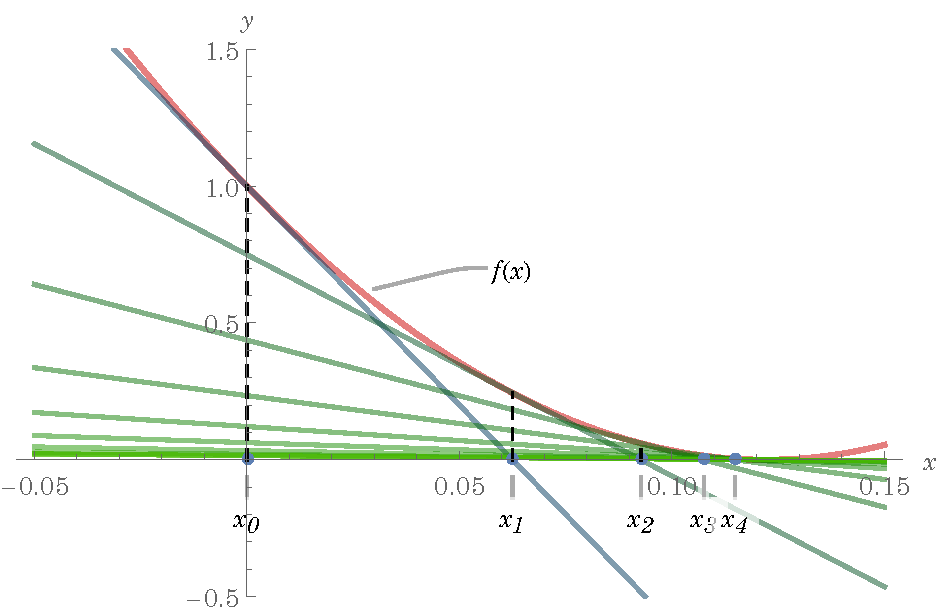
\includegraphics[scale = 0.8]{Figure/Newton1.pdf}
        \label{figure:Newton1}
    \end{subfigure}
    \caption{Newton 法迭代结果 1 }
    \label{Newton1}
\end{figure}
\begin{figure}
    \centering
    \begin{subfigure}[t]{\textwidth}
        \centering
        \begin{tabular}{|l|c|c|}
            \hline
            迭代步数$k$            & $x_k$                        & $f(x_k)$                     \\
            \hline $k = 0$(初值) & $3.0000000000\text{E}{+}000$ & $1.3120000000\text{E}{+}003$ \\
            \hline $k = 1$         & $1.9192751236\text{E}{+}000$ & $3.9180729077\text{E}{+}002$ \\
            \hline $k = 2$         & $1.1936133228\text{E}{+}000$ & $1.1368262566\text{E}{+}002$ \\
            \hline $k = 3$         & $7.3112145458\text{E}{-}001$ & $3.1859876182\text{E}{+}001$ \\
            \hline $k = 4$         & $4.5362080609\text{E}{-}001$ & $8.6190504416\text{E}{+}000$ \\
            \hline $k = 5$         & $2.9663693142\text{E}{-}001$ & $2.2633471161\text{E}{+}000$ \\
            \hline $k = 6$         & $2.1197535112\text{E}{-}001$ & $5.8197426653\text{E}{-}001$ \\
            \hline $k = 7$         & $1.6779403531\text{E}{-}001$ & $1.4770709460\text{E}{-}001$ \\
            \hline $k = 8$         & $1.4519438879\text{E}{-}001$ & $3.7206334228\text{E}{-}002$ \\
            \hline $k = 9$         & $1.3376760731\text{E}{-}001$ & $9.3253679860\text{E}{-}003$ \\
            \hline $k = 10$        & $1.2803649704\text{E}{-}001$ & $2.3222638207\text{E}{-}003$ \\
            \hline $k = 11$        & $1.2519603327\text{E}{-}001$ & $5.6755417123\text{E}{-}004$ \\
            \hline $k = 12$        & $1.2383872242\text{E}{-}001$ & $1.2927049695\text{E}{-}004$ \\
            \hline $k = 13$        & $1.2327102895\text{E}{-}001$ & $2.2587102744\text{E}{-}005$ \\
            \hline $k = 14$        & $1.2311856261\text{E}{-}001$ & $1.6284754711\text{E}{-}006$ \\
            \hline $k = 15$        & $1.2310571808\text{E}{-}001$ & $1.1556329893\text{E}{-}008$ \\
            \hline $k = 16$        & $1.2310562562\text{E}{-}001$ & $5.9885429948\text{E}{-}013$ \\
            \hline \multicolumn{3}{|c|}{$|f(x_{16})| < \varepsilon$,停止迭代}                   \\
            \hline
        \end{tabular}
        \label{table:Newton2}
    \end{subfigure}
    \begin{subfigure}[t]{\textwidth}
        \centering
        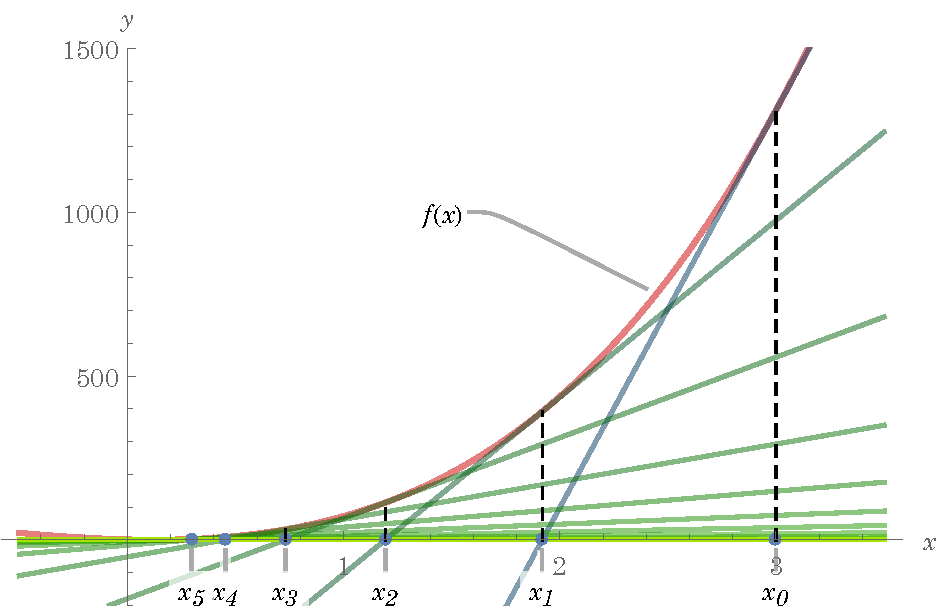
\includegraphics[scale = 0.8]{Figure/Newton2.pdf}
        \label{figure:Newton2}
    \end{subfigure}
    \caption{Newton 法迭代结果 2 }
    \label{Newton2}
\end{figure}
\begin{figure}
    \centering
    \begin{subfigure}[t]{\textwidth}
        \centering
        \begin{tabular}{|l|c|c|}
            \hline
            迭代步数$k$            & $x_k$                         & $f(x_k)$                     \\
            \hline $k = 0$(初值) & $+0.0000000000\text{E}{+}000$ & $1.0000000000\text{E}{+}000$ \\
            \hline $k = 1$(初值) & $+5.0000000000\text{E}{-}001$ & $1.1375000000\text{E}{+}001$ \\
            \hline $k = 2$         & $-4.8192771084\text{E}{-}002$ & $1.9100839450\text{E}{+}000$ \\
            \hline $k = 3$         & $-1.5882177241\text{E}{-}001$ & $4.9849583298\text{E}{+}000$ \\
            \hline $k = 4$         & $+2.0528956326\text{E}{-}002$ & $6.9745241532\text{E}{-}001$ \\
            \hline $k = 5$         & $+4.9704099508\text{E}{-}002$ & $3.5839401507\text{E}{-}001$ \\
            \hline $k = 6$         & $+8.0543024888\text{E}{-}002$ & $1.1965360731\text{E}{-}001$ \\
            \hline $k = 7$         & $+9.5999095782\text{E}{-}002$ & $4.7582804260\text{E}{-}002$ \\
            \hline $k = 8$         & $+1.0620354980\text{E}{-}001$ & $1.7777847602\text{E}{-}002$ \\
            \hline $k = 9$         & $+1.1229022963\text{E}{-}001$ & $6.8102183582\text{E}{-}003$ \\
            \hline $k = 10$        & $+1.1606968076\text{E}{-}001$ & $2.5795784215\text{E}{-}003$ \\
            \hline $k = 11$        & $+1.1837415259\text{E}{-}001$ & $9.7415265691\text{E}{-}004$ \\
            \hline $k = 12$        & $+1.1977247782\text{E}{-}001$ & $3.6072356011\text{E}{-}004$ \\
            \hline $k = 13$        & $+1.2059475518\text{E}{-}001$ & $1.2741741436\text{E}{-}004$ \\
            \hline $k = 14$        & $+1.2104383231\text{E}{-}001$ & $3.9878767168\text{E}{-}005$ \\
            \hline $k = 15$        & $+1.2124841215\text{E}{-}001$ & $9.3453570276\text{E}{-}006$ \\
            \hline $k = 16$        & $+1.2131102788\text{E}{-}001$ & $1.1695181286\text{E}{-}006$ \\
            \hline $k = 17$        & $+1.2131998479\text{E}{-}001$ & $4.4816937383\text{E}{-}008$ \\
            \hline $k = 18$        & $+1.2132034170\text{E}{-}001$ & $2.3240176450\text{E}{-}010$ \\
            \hline \multicolumn{3}{|c|}{$|f(x_{18})| < \varepsilon$,停止迭代}                    \\
            \hline
        \end{tabular}
        \label{table:Secant1}
    \end{subfigure}
    \begin{subfigure}[t]{\textwidth}
        \centering
        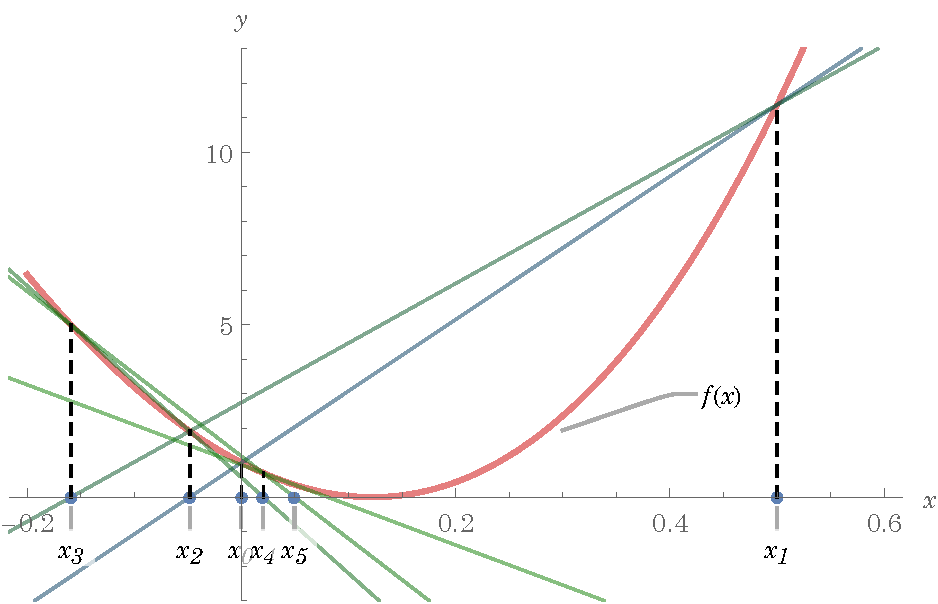
\includegraphics[scale = 0.8]{Figure/Secant1.pdf}
        \label{figure:Secant1}
    \end{subfigure}
    \caption{弦截法迭代结果 1 }
    \label{Secant1}
\end{figure}
\begin{figure}
    \centering
    \begin{subfigure}[t]{.65\textwidth}
        \centering
        \begin{tabular}{|l|c|c|}
            \hline
            迭代步数$k$            & $x_k$                        & $f(x_k)$                     \\
            \hline $k = 0$(初值) & $1.0000000000\text{E}{-}001$ & $3.4200000000\text{E}{-}002$ \\
            \hline $k = 1$(初值) & $1.5000000000\text{E}{+}000$ & $2.0537500000\text{E}{+}002$ \\
            \hline $k = 2$         & $9.9766826661\text{E}{-}002$ & $3.4920022729\text{E}{-}002$ \\
            \hline $k = 3$         & $9.9528703766\text{E}{-}002$ & $3.5662994682\text{E}{-}002$ \\
            \hline $k = 4$         & $1.1095871197\text{E}{-}001$ & $8.7722830757\text{E}{-}003$ \\
            \hline $k = 5$         & $1.1468740718\text{E}{-}001$ & $3.8969392942\text{E}{-}003$ \\
            \hline $k = 6$         & $1.1766781216\text{E}{-}001$ & $1.3876451955\text{E}{-}003$ \\
            \hline $k = 7$         & $1.1931598272\text{E}{-}001$ & $5.3099453171\text{E}{-}004$ \\
            \hline $k = 8$         & $1.2033760050\text{E}{-}001$ & $1.9023231922\text{E}{-}004$ \\
            \hline $k = 9$         & $1.2090792407\text{E}{-}001$ & $6.3397280115\text{E}{-}005$ \\
            \hline $k = 10$        & $1.2119299484\text{E}{-}001$ & $1.7038550552\text{E}{-}005$ \\
            \hline $k = 11$        & $1.2129776891\text{E}{-}001$ & $2.8550135170\text{E}{-}006$ \\
            \hline $k = 12$        & $1.2131885895\text{E}{-}001$ & $1.8556909953\text{E}{-}007$ \\
            \hline $k = 13$        & $1.2132032505\text{E}{-}001$ & $2.3119210990\text{E}{-}009$ \\
            \hline $k = 14$        & $1.2132034354\text{E}{-}001$ & $1.9196866319\text{E}{-}012$ \\
            \hline \multicolumn{3}{|c|}{$|f(x_{14})| < \varepsilon$,停止迭代}                   \\
            \hline
        \end{tabular}
        \label{table:Secant2}
    \end{subfigure}
    \begin{subfigure}[t]{.33\textwidth}
        \centering
        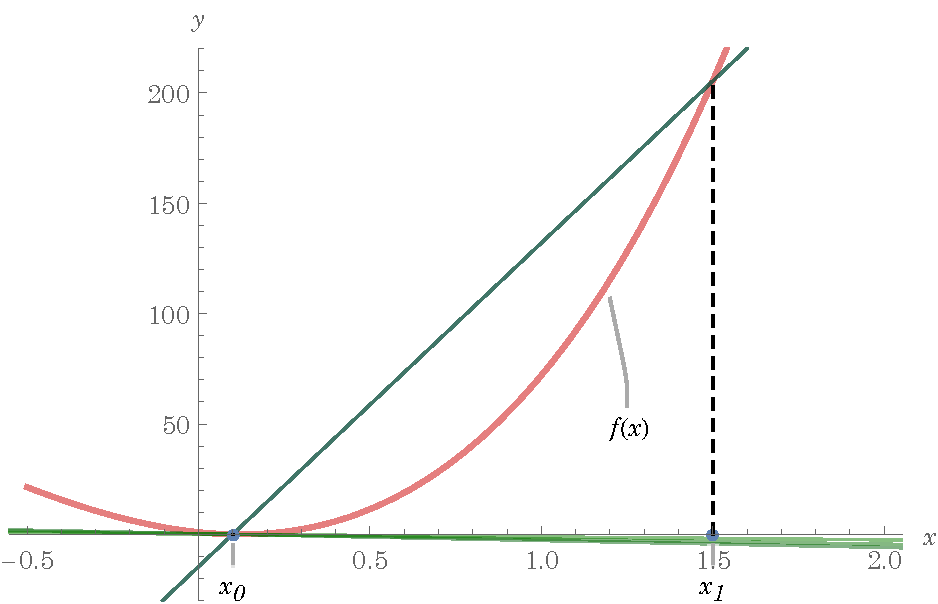
\includegraphics[scale = 0.33]{Figure/Secant2.pdf}
        \caption{整体示意图}
        \label{figure:Secant2}
    \end{subfigure}
    \begin{subfigure}[t]{\textwidth}
        \centering
        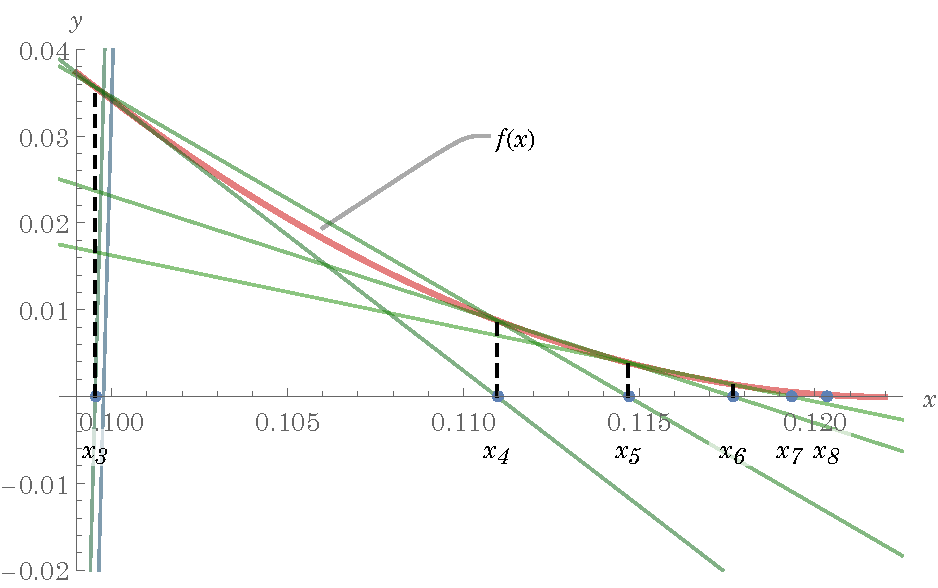
\includegraphics[scale = 0.8]{Figure/Secant2-zoom.pdf}
        \caption{局部放大图}
        \label{figure:Secant2-zoom}
    \end{subfigure}
    \caption{弦截法迭代结果 2 }
    \label{Secant2}
\end{figure}

\section{结果分析}


\section{算法分析}


\section{实验结论}

\end{document}
